\documentclass{beamer}
\usetheme[navigation]{UMONS}
\usepackage[utf8]{inputenc}
\usepackage[english]{babel}
\newcommand{\slideheight}{7cm}
\newcommand{\slidewidth}{12cm}
\newcommand{\incicon}[1]{\includegraphics[height=0.7cm]{figures/#1}}

\title[Google File System]{The Google File System}
\author[B.Jason]{Jason \textsc{Bury}}
\institute[UMons-FS]{%
 Faculté des Sciences\\
  Université de Mons
  \\[2ex]
  
\includegraphics[height=4ex]{figures/UMONS}\hspace{2em}%
  \raisebox{-1ex}{
\includegraphics[height=6ex]{figures/UMONS_FS}}
}

\begin{document}
\maketitle

\section{Introduction}
\subsection{Introduction}
% Hello everybody, I will introduce you the Google's paper about their new File System.
% A Google file system is generally used by thousands of users that want to share a huge amount of data
% A Google's team observed common problems and application behaviors to design a new file system more adapted to their client's application.
\begin{frame}
 \frametitle{The Google File System}
 \alert{One} file system for \alert{thousands} users\\
 \centering
 \includegraphics[height=6.5cm]{figures/terregfsschema.png}
\end{frame}

% Here are some problems they had to manage:
%  -The need of data processing is rapidly growing
%  -There are thousands of inexpensive storage machines used by thousands of clients.
%   So many that At any time, there is a componenent failure and it can to not recover.
%  -The files are huge, typically multi-GB
%  -The common files mutation here is data appending at the end of the file.
%   Writes within a file are very rare.
\begin{frame}
 \frametitle{The problems}
 \begin{itemize}
  \item \incicon{NPenhancement.png} Growing demands of data processing
  \item \incicon{NPbrokenDisc.png} Component failures
  \item \incicon{NPbigdataBlack.png} Huge files
  \item \incicon{NPpiled.png} Many appends
  \item \incicon{stream.png} Large streaming reads
 \end{itemize}
\end{frame}

% About unavoidable failures, Here are the main ideas to maintain a fault tolerance:
% Data replication will ensure that client still have access to their data even if a file is corrupted or unavailable.
% To continue to treat the big flow of client request, servers must be operational as fast as possible.
% A log system ensure that no data will be lost even if a fail occur during a mutation
% Then, data integrity is assured for the client (but not for a server) thanks to checksum and version number.
% We will see how they integrated these in the system but also how they deal with the big amout of client request and especially append request.
\begin{frame}
 \frametitle{Fault tolerance}
 \begin{itemize}
  \item \alert{Data replication}
  \item \alert{Fast recovery} (fast reboot)
  \item \alert{Log system}
  \item \alert{Data integrity} (checksum + version number)
 \end{itemize}
\end{frame}

\section{Architecture}
\subsection{Architecture}
% The file system is distributed across multiple servers.
% All the files data are stored in chunkservers
% A master server process all client's first request and is in charge of maintenance for the file system.
\begin{frame}
 \frametitle{One Master, thousands chunkservers}
 \centering
 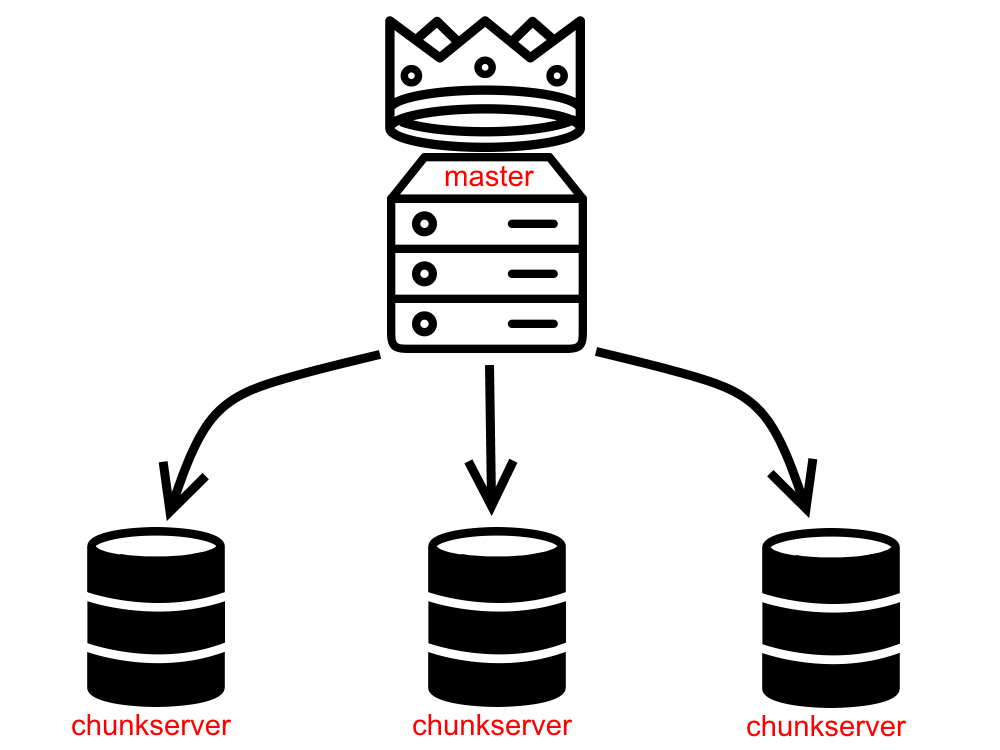
\includegraphics[height=\slideheight]{figures/masterschema.png}
\end{frame}

% Files are splitted into one or several sixty-four Megabytes chunks.
% All chunks are replicated at least 3 times.
% The numbers of replica is chosen by the client.
% Then all replicas are stored in different chunkserver.
% So, the client lose access to its data only if all these chunkserver fails at the same time.
% and this case is unlikely from 3 replicas.
% Thanks to this, the system can also support files larger than the storage capacity of a server.
\begin{frame}
 \frametitle{A file}
 \centering
 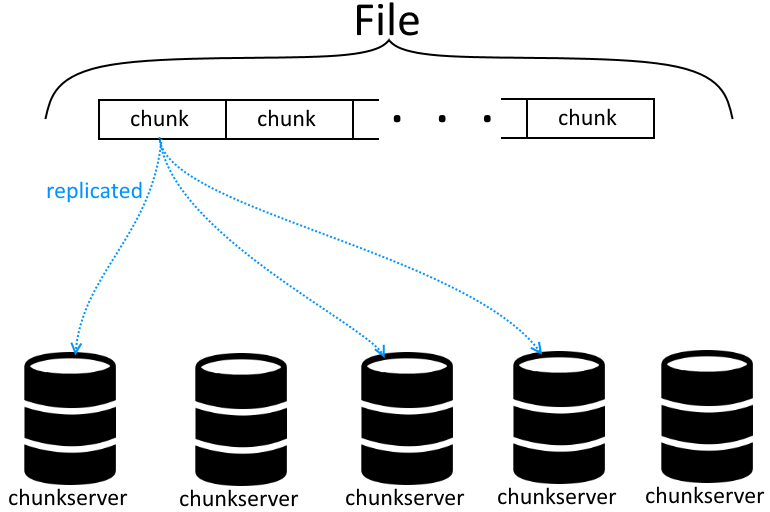
\includegraphics[height=\slideheight]{figures/filegfsschema.png}
\end{frame}

\newcommand{\masterpicheight}{5cm}
% The master contains all metadatas about the file system.
% These metadatas allow the user to find desired files ande are stored in three data structures.
% Firstly, all file names are mapped to the list of unique IDs of their chunks. 
\begin{frame}
 \frametitle{What is in the master ?}
 \framesubtitle{The file mapping}
 \centering
 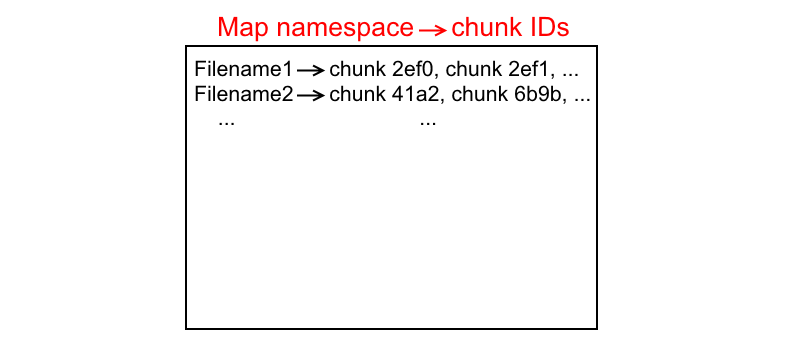
\includegraphics[height=\masterpicheight]{figures/namespaceMapschema.png}
\end{frame}

% Then, another mapping maps chunk IDs to the location of their replicas
\begin{frame}
 \frametitle{What is in the master ?}
 \framesubtitle{The chunk mapping}
 \centering
 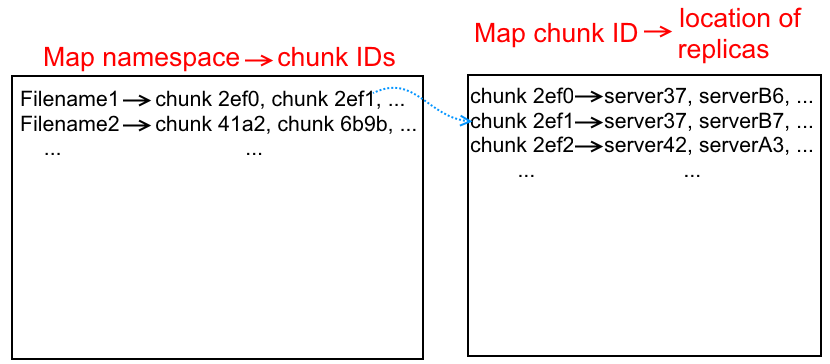
\includegraphics[height=\masterpicheight]{figures/namespaceMapMapschema.png}
\end{frame}

% And, To allow us to explore files like in i-node system,
% A tree organizes the files and their name correspond to the namespace in the tree.TODO correct ?
\begin{frame}
 \frametitle{What is in the master ?}
 \framesubtitle{The namespace tree}
 \centering
 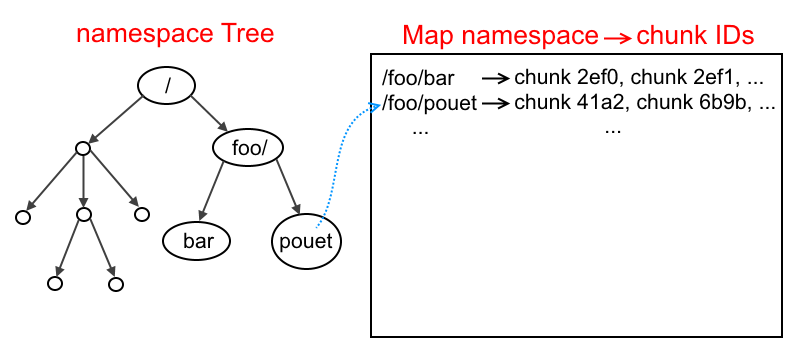
\includegraphics[height=\masterpicheight]{figures/namespaceTreeMapschema.png}
\end{frame}

% All metadata changes are logged in a file so that the master can recover after a fail.
% If the change is due to a client request, the log is written before responding to the client.
% The master recovers the file system by replaying the operations log.
% Regular checkpoints allow fast recovery by assuring that operations logged before the checkpoints are performed.
% The log is stored in remote servers.
\begin{frame}
 \frametitle{The operations Log}
 \begin{center}
 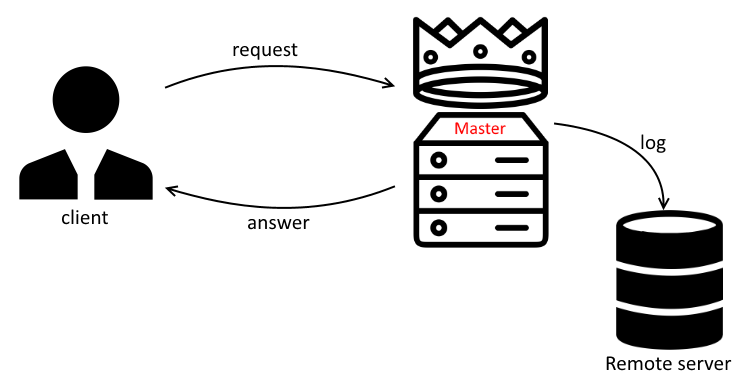
\includegraphics[height=6cm]{figures/logschema.png}
 \alert{+ checkpoints}\\
 $\Rightarrow$ fast recovery
 \end{center}
\end{frame}

\section{Interactions}
\subsection{Interactions}
% Now, we will see the interactions between clients, chunkservers and the master to read or write a file.
% For a read,
% The client asks to the master,
% the location of a replica of a chunk providing the file name and the chunk index computed from chunk size and the offset.
% After assuring that all replicas are available,
% the master responds with the chunk ID and the location of all replicas.
% No more interactions is needed between the client and the master.
% The client sends its request to one of the chunkservers containing the desired replica and data is transfered.
% If the replica is not available at this moment, the client sends the request again to another chunkserver containing the replica.
\begin{frame}
 \frametitle{Interactions for a read}
 \centering
 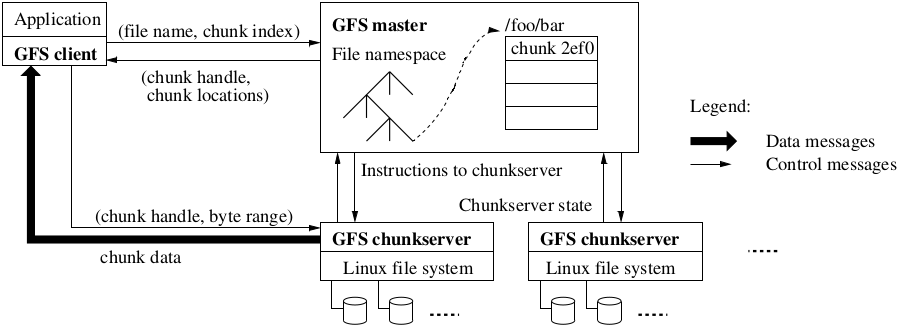
\includegraphics[width=\slidewidth]{figures/GFSarchitecture.png}
\end{frame}

% If we want to write, The write has to be made at all chunk replicas.
% First of all, the master grants one of the chunkservers containing a replica of the chunk to mutate.
% This chunkserver is called the primary.
% So, step1, the client asks to the master which chunkserver is the primary and the location of chunk replicas.
% Step 2, the master responds and the client caches the primary identity
% so that, for future mutations to the chunk,
% no more interactions between the client and the master is needed until the primary becomes unreachable.
% Step 3, the data is transfered to the chunkservers.
% The maner that the data is transfered depends on the network topology and bandwith.
% Step 4, its time to write the data in the persistent memory:
% The client sends a write request to the primary.
% The primary can receive multiple write requests for the same chunk concurrently from different clients.
% It assigns a serial number to all these request to define the order of mutation to do.
% Step 5, the primary sends the write request to secondary chunkservers providing the sequence of serial numbers.
% Then, step 6, all secondaries indicate to the primary that the operation is complete or failed.
% Finally, the primary indicates to the client if the write is a success or it failed in a secondary replica.
% If it failed, it loops starting at the third step were the client sends data to the secondary chunkservers that failed the operation.
% And if the fail still occur after some iterations of the loop, the client restarts at step 1.
\begin{frame}
 \frametitle{Interactions for a write}
 \centering
 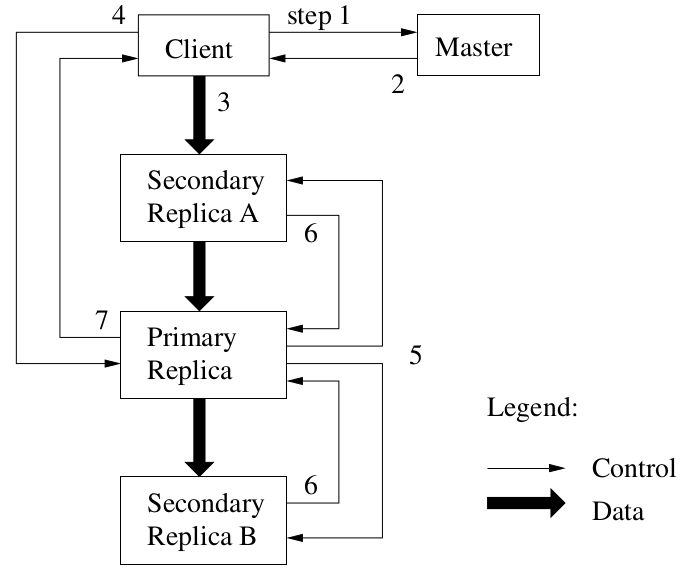
\includegraphics[height=\slideheight]{figures/GFSflow.png}
\end{frame}

% The random write in the same region can't be concurrent
% But if the write is an append, then the client doesn't have to inform the region where to write.
% The Google File System choose the offset where to write the append and this allow it to perform the write concurrently.
% without synchronisation by locks.
% The writing is performed as a multiple-producer/single-consumer queue.
\begin{frame}
 \frametitle{The append operation}
 Concurrent appends in \alert{one} operation\\\vspace{0.5cm}
 \centering
 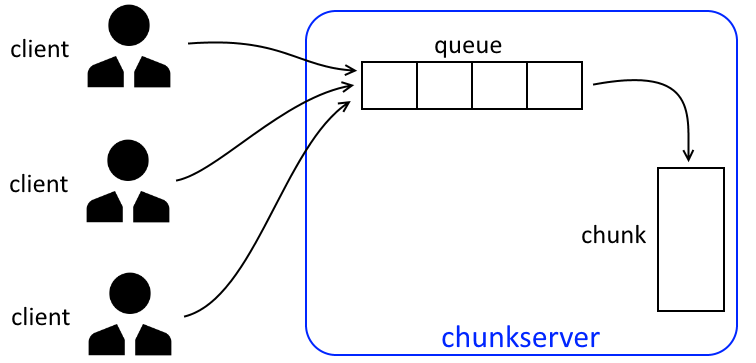
\includegraphics[width=11cm]{figures/appendsschema.png}
\end{frame}

% If the data in the chunk + the append will exceed the maximum chunk size,
% The primary pads the chunk to the maximum size, tell to secondaries to do the same,
% and asks to the client to do the append on the next chunk.
\begin{frame}
 \frametitle{The append operation}
 \framesubtitle{Data that exceeds chunk}
 \centering
 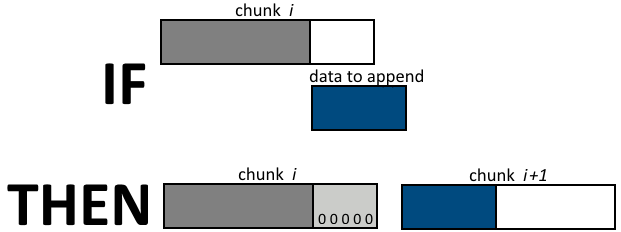
\includegraphics[width=\slidewidth]{figures/appends2schema.png}
\end{frame}

\section{Master's operations}
\subsection{Master operations}

% The master is in charge of , among others, Replica placement,
% replica creation, displacement and deletion
% and garbage collection
\begin{frame}
 \frametitle{Master operations}
 \begin{itemize}
  \item \alert{Replica placement}
  \item \alert{Re-replica} (creation and copy of replica)
  \item \alert{Rebalancing} (displacement of replica)
  \item \alert{Garbage collection}
 \end{itemize}
\end{frame}

% The master places the replicas of a chunk in chunksever from different racks.
% So, even if a power supply or a switch fails, the client still have access to its data.
% Also, since chunkservers in a rack are connected to the same switch,
% The bandwith is higher if we use the aggregate bandwith of three racks instead of three chunkservers bottlenecked by their common switch.
\begin{frame}
 \frametitle{Replica placement}
 In different racks\\\vspace{0.3cm}
 \centering
 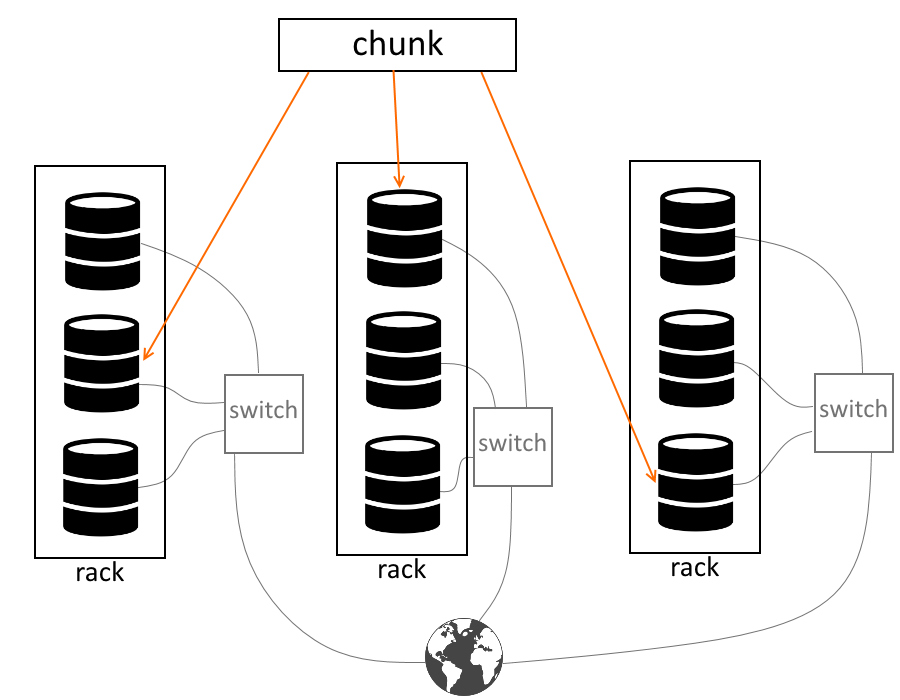
\includegraphics[height=6cm]{figures/racksschema.png}
\end{frame}

% The master can also decides to create or displace a replica.
% The reasons are: chunk creation by the client,
% Or a replica is anavailable and so we have to create the missing replica
% Or just to balance bandwith use among servers
\begin{frame}
 \frametitle{Re-replica and rebalancing}
 There are 3 reasons that a replica is created:
 \begin{enumerate}
  \item The chunk is just created.
  \item The number of replicas is below an user-specified goal.
  \item The master moves it for better load balancing.
 \end{enumerate}
\end{frame}

% The garbage collector is a regular scan of the file system.
% it removes replicas deleted by a client, corrupted or stale replicas and orphan chunks
\begin{frame}
 \frametitle{Garbage collection}
 It cleans up:
 \begin{itemize}
  \item Chunk replicas deleted by a client
  \item Corrupted replicas using checksum
  \item Stale replicas using version number
  \item Orphan chunks
 \end{itemize}
\end{frame}

% When the client requests to remove a file,
% The master just renames it to a hidden name.
% The scan of the file system remove these renamed files 3 days after the client request.
% This remove does not concern data in the chunk server but only in the metadatas.
\begin{frame}
 \frametitle{Garbage collection}
 \framesubtitle{Removing file}
 \centering
 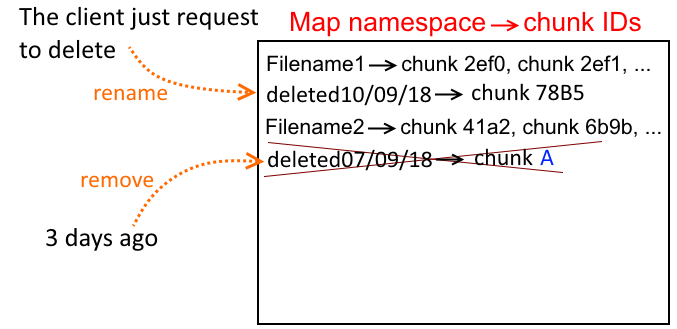
\includegraphics[width=\slidewidth]{figures/removeschema.png}
\end{frame}

% Chunkserver send regular heartbeat message to the master containing a subset of chunk IDs that the chunkserver store.
% The master responds with the list of unknown chunk IDs, tipycally the IDs of removed chunks,
% To allow the chunkserver to delete chunks in their persistent memory.
\begin{frame}
 \frametitle{Garbage collection}
 \framesubtitle{Recover memory}
 \centering
 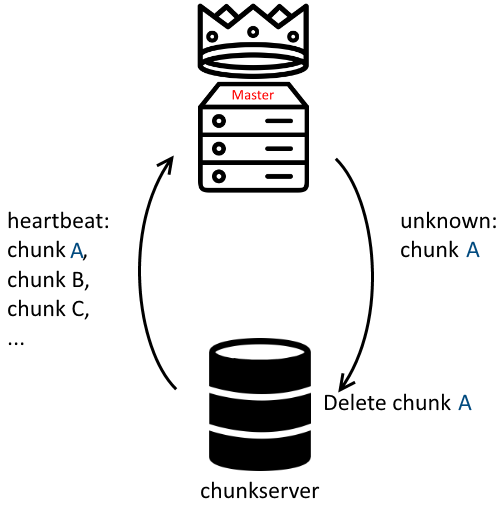
\includegraphics[height=\slideheight]{figures/recoverymemoryschema.png}
\end{frame}

% During the scan, the master also clean up chunks that are in the mapping of chunk IDs and their location
% that are not in the file-to-chunk mappings.
\begin{frame}
 \frametitle{Garbage collection}
 \framesubtitle{Orphan chunks}
 \centering
 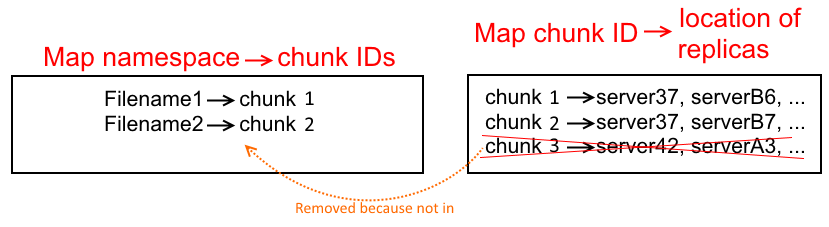
\includegraphics[width=\slidewidth]{figures/orphanschema.png}
\end{frame}

% A chunk replica may become stale if a chunkserver misses a mutation request.
% That's why each chunks contains a version number to distinguish up-to-date replicas.
% Then, the master can detect stale replicas during the garbage collection and it deletes them.
% Moreover, if a chunkserver restart, it sends immediatly to the master which chunks it stores and with their version number.
\begin{frame}
 \frametitle{Garbage collection}
 \frametitle{Stale replica detection}
 If mutation missed\\
 ~~$\Rightarrow$~~stale replica\\
 ~~$\Rightarrow$~~Version number not updated\\
 ~~$\Rightarrow$~~Detected during garbage collection or chunserver reboot
\end{frame}

% The chunkserver compute a checksum according to received data before writing it data in persistent memory.
% Let's assume that the hard drive failed and so, the writen data doesn't match the checksum
% The only moment when the corruption is detected is when the chunkserver receive a read request.
% Because at this time, it computes the checksum of stored data before sending it.
% If the corruption is detected, an error is send instead of the data and the master will remove the replica.
\begin{frame}
 \frametitle{Garbage collection}
 \frametitle{Corrupted replica detection}
 If mutation incorrect\\
 ~~$\Rightarrow$~~corrupted replica\\
 ~~$\Rightarrow$~~Checksum not corresponding to data\\
 ~~$\Rightarrow$~~Detected after a read request\\
 ~~$\Rightarrow$~~Error message send\\
 ~~$\Rightarrow$~~Master warned\\
 ~~$\Rightarrow$~~replica deleted
\end{frame}

\section{Rate measurements}
\subsection{Measurements}
\newcommand{\ratemesoption}{7cm}
\newcommand{\ratemehspace}{\hspace{15mm}}
% As a conclusion, I will show you some result of their test before deployment.
% They measured the aggregate read rate of 16 clients on 16 chunkservers.
% In the graphic here, the first curve is the theorical maximum agregate rate estimated following the network limit.
% The second curve is, of course, the measured rate.
% We can see that the rate is increasing but more and more slowly to reach an asymptote: the theorical maximum that is 125MB/s
% The increase is more and more slowly because the more readers the more probability of concurrent reading
\begin{frame}
 \frametitle{Read rate}
 \ratemehspace
 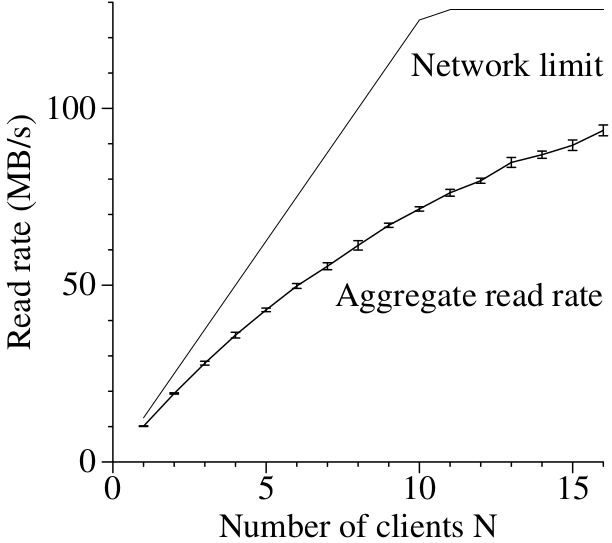
\includegraphics[height=\ratemesoption]{figures/GFSreads.png}
\end{frame}

% The curve shape is the same for aggregate random write rate.
% except that the theorical maximum stagnates to 67MB/s here and the rate is increasing even slower.
% Because the data have to be transfered to 3 chunkservers for each writes,
% we have a lower maximum rate.
% Also, the asymptote here is about the half of the maximum theorical rate.
% It is due to their network stack.
% It doesn't interact very well with their pipelining scheme.
% But because random write are very rare, we should not be worry about.
\begin{frame}
 \frametitle{Write rate}
 \ratemehspace
 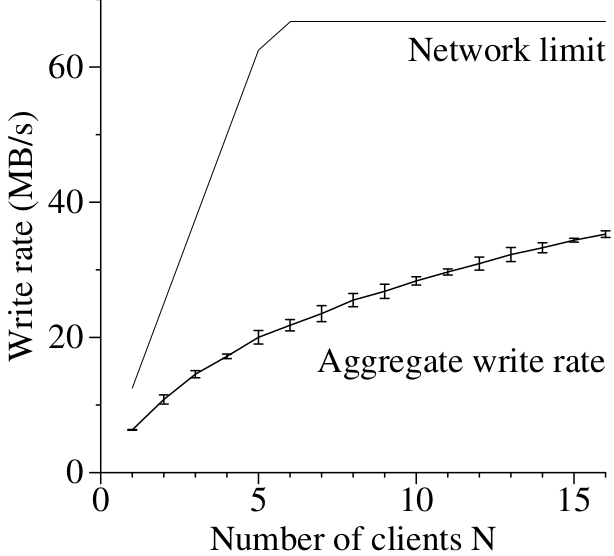
\includegraphics[height=\ratemesoption]{figures/GFSwrites.png}
\end{frame}

% Finally, the aggregate append write rate.
% All clients appends data to the same file.
% Then, the network limit falls to 12MB/s because the bandwith is limited to that of the chunkserver.
% Because of the same reason, the aggregate rate is not clearly increasing or decreasing.
% The variation is due to network congestion.
\begin{frame}
 \frametitle{Append rate}
 \ratemehspace
 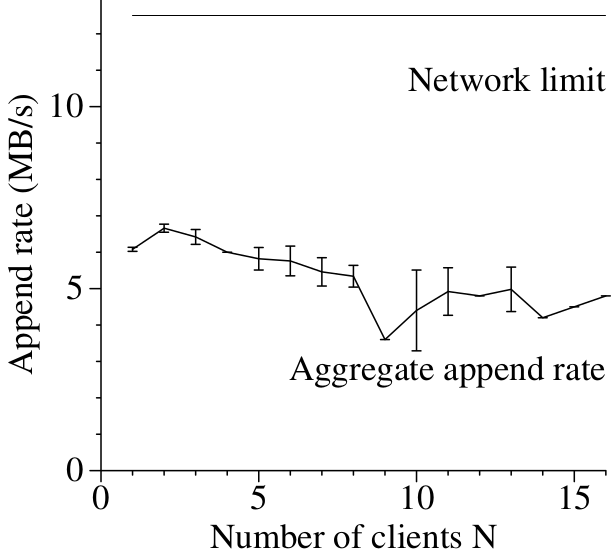
\includegraphics[height=\ratemesoption]{figures/GFSappends.png}
\end{frame}

% In conclusion, we have fault-tolerant system
% That can store file even larger than storage discs
% and efficient for large streaming reads and concurrent appends
\newcommand{\inccheck}{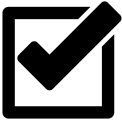
\includegraphics[scale=0.08]{figures/checkalvareduce.png}~}
\begin{frame}
 \frametitle{Conclusion}
 \begin{itemize}
  \item[] \inccheck Fault-tolerant
  \item[] \inccheck For huge files
  \item[] \inccheck Efficient for large streaming reads
  \item[] \inccheck Efficient for concurrent appends
 \end{itemize}
\end{frame}

\end{document}